

\noindent 
\textbf{\stepcounter{zadatak}
\thecjelina.\thezadatak.}
Na blok mase $m = 2\ kg$ djelujemo silom $F = 25,0\ N$
usporedno s nagibom kosine (kao na slici). Ako je kosina
nagiba $\alpha = 39^\circ$, a koeficijent kineti\v{c}kog trenja između
bloka i podloge $\mu_k = 0,25$ koliko je ubrzanje bloka?
\begin{figure}[ht]%{r}{0.3\textwidth} % Inline image example
  \begin{center}
    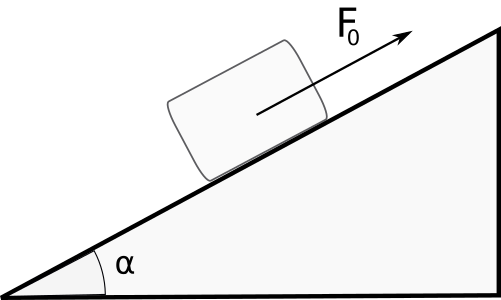
\includegraphics[width=0.3\textwidth]{03_Dinamika_materijalne_tocke/kosina.png}
  \end{center}
  %\caption{Fish}
\end{figure}

